\documentclass[11pt]{article}
\usepackage[utf8]{inputenc}
\usepackage[T1]{fontenc}
\usepackage[spanish,es-nodecimaldot]{babel}
\usepackage{amsmath,amssymb,amsthm}
\usepackage{graphicx,booktabs,longtable,tabularx,array,enumitem,geometry,xcolor,float}
\usepackage{hyperref}
\usepackage{mathptmx}
\geometry{top=2.1cm,bottom=2.1cm,left=2.15cm,right=2.15cm}
\hypersetup{colorlinks=true,linkcolor=blue!45!black,citecolor=blue!45!black,urlcolor=blue!55!black}
\setlength{\parindent}{1.25em}
\setlength{\parskip}{0.15em}
\setlength{\tabcolsep}{4pt}
\emergencystretch=3em

\title{\bfseries Influencia del crecimiento y del umbral de carga\\
\large Tablas hash dinámicas con hashing universal}
\author{José Cisternas \and Gabriel Olarte \and Bernardo del Aguila \and Wara Murillo\\
\normalsize Algorítmica II -- Universidad Privada Boliviana}
\date{11 de septiembre de 2026}

\begin{document}
\maketitle

\begin{abstract}
Este trabajo estudia cómo el factor multiplicativo de crecimiento $\gamma$ y el umbral de carga $\tau$ modifican el costo amortizado, la memoria y las colisiones de una tabla hash dinámica. Se implementó en Python una tabla con encadenamiento separado, redimensionamiento geométrico y una familia universal modular; como contraste, se adaptó una tabla con sondeo lineal. El diseño factorial evaluó cinco factores de crecimiento, cuatro umbrales, tres tamaños de instancia y 30 repeticiones independientes, para 1800 ejecuciones principales. En $N=100000$, aumentar $\gamma$ de 1.25 a 4 redujo las migraciones medias de 4.508 a 0.723 por inserción, mientras elevó la memoria estructural final de 157.7 a 276.8 bytes por elemento. La correlación de rangos entre $\gamma$ y migraciones fue $-1.000$; entre $\tau$ y pares que colisionan fue 0.949. El cociente medio entre colisiones observadas y la cota esperada universal fue 0.964. Los resultados respaldan el compromiso previsto: crecer más reduce reconstrucciones, pero reserva más memoria; un umbral alto incrementa la carga y las colisiones. No existe una configuración óptima independiente del objetivo y del entorno.
\end{abstract}

\noindent\textbf{Palabras clave:} hashing universal; análisis amortizado; tablas hash dinámicas; colisiones; reproducibilidad.

\section{Introducción}
Las tablas hash proporcionan acceso eficiente cuando las claves se distribuyen adecuadamente. En una implementación dinámica, sin embargo, no basta con elegir una función de dispersión: también debe decidirse cuándo reconstruir la tabla y cuánto crecer. Un crecimiento pequeño conserva espacio, pero repite migraciones; uno grande reduce reconstrucciones, aunque deja capacidad ociosa. De manera análoga, un umbral bajo acorta cadenas a costa de reservar más buckets.

El problema es algorítmicamente relevante porque combina dos tipos de garantía que suelen confundirse. El costo amortizado distribuye el trabajo de reconstrucciones ocasionales sobre una secuencia completa, sin suponer una distribución probabilística. El hashing universal, en cambio, ofrece una esperanza respecto de la función seleccionada aleatoriamente \cite{CarterWegman1979,Tarjan1985}. La brecha que abordamos es observar ambas garantías en una misma implementación instrumentada, manteniendo separadas sus unidades de medida.

\subsection{Pregunta de investigación}
¿Cómo influyen el factor de redimensionamiento $\gamma$ y el umbral de carga $\tau$ en las migraciones amortizadas, el consumo de memoria y el número esperado de colisiones de una tabla hash dinámica con hashing universal?

\subsection{Hipótesis o expectativa contrastable}
\textbf{H1.} Al aumentar $\gamma$ disminuirán el número de redimensionamientos y las migraciones por inserción aproximadamente como $1/(\gamma-1)$, pero aumentarán la reserva y el pico de memoria. Al aumentar $\tau$ crecerán la carga y las colisiones. Las métricas formarán una frontera de compromiso, no un ganador universal.

\textbf{H0.} Una vez controlada la carga realizada $\alpha$, $\gamma$ y $\tau$ no producirán un efecto directo adicional sobre los pares que colisionan; los residuos se explicarán por trayectoria, redondeo a primos y variabilidad entre funciones hash.

\subsection{Contribuciones}
\begin{itemize}[leftmargin=1.5em]
\item \textbf{Teórica:} una derivación que distingue migraciones amortizadas, colisiones esperadas y promedios empíricos.
\item \textbf{Experimental:} un factorial reproducible de 1800 ejecuciones, métricas separadas, intervalos bootstrap y ocho visualizaciones finales.
\item \textbf{Integración:} una matriz completa del bloque final y un contraste con sondeo lineal que evita trasladar métricas entre esquemas incompatibles.
\end{itemize}

\section{Trabajos relacionados / estado del arte}
Carter y Wegman introducen familias universales para controlar colisiones sin asumir claves aleatorias \cite{CarterWegman1979}. Tarjan organiza el análisis amortizado de secuencias \cite{Tarjan1985}, mientras Larson relaciona carga, expansión y reorganización en tablas dinámicas \cite{Larson1988}. Estos trabajos fundamentan las variables principales, pero no determinan una política única para una implementación moderna.

Otros esquemas muestran por qué las conclusiones dependen de la representación. El hashing perfecto dinámico busca consultas de peor caso \cite{DietzfelbingerEtAl1994}; cuckoo hashing usa reconstrucción aleatoria ante ciclos \cite{PaghRodler2004}; el análisis de sondeo lineal revela una dependencia pronunciada de la carga \cite{FlajoletPobleteViola1998}. La independencia requerida también cambia según la aplicación \cite{PatrascuThorup2012}.

La literatura reciente estudia alta carga, concurrencia y arquitectura: DyCuckoo se orienta a GPU \cite{LiEtAl2021}, Iceberg hashing optimiza varios criterios simultáneos \cite{BenderEtAl2023}, y los benchmarks vectorizados evidencian que el hardware puede alterar los rankings \cite{BoetherEtAl2023}. Los arreglos redimensionables delimitan, además, la frontera tiempo--espacio del crecimiento geométrico \cite{BrodnikEtAl1999,TarjanZwick2024}.

\subsection{Síntesis crítica}
La evidencia converge en tres puntos: la carga afecta las colisiones, la reconstrucción distribuye un costo ocasional y ninguna política domina todas las métricas. No obstante, las garantías de encadenamiento, sondeo lineal, cuckoo hashing y estructuras para GPU no son intercambiables. Nuestro estudio no intenta reproducir cada arquitectura; aísla $\gamma$ y $\tau$ en una implementación controlada y usa los demás enfoques como contexto o contraste.

\section{Fundamento teórico y algoritmos}
\subsection{Modelo del problema}
La entrada es una secuencia de $N$ claves enteras únicas y un tratamiento $(\gamma,\tau)$, con $\gamma>1$ y $0<\tau<1$. La tabla tiene $m$ buckets, $n$ elementos y carga $\alpha=n/m$. La salida experimental es un vector de métricas: migraciones, redimensionamientos, comparaciones, pares que colisionan, memoria y tiempo. Las semillas de claves, orden y hash se registran por separado.

La familia usada es
\[
h_{a,b}(x)=((ax+b)\bmod p)\bmod m,
\qquad p=2^{61}-1,
\]
con $a\in\{1,\ldots,p-1\}$ y $b\in\{0,\ldots,p-1\}$. En cada reconstrucción se renuevan $(a,b)$. Para longitudes de cadena $L_j$, el conteo de pares es
\[
C_{\mathrm{pares}}=\sum_{j=0}^{m-1}\binom{L_j}{2},
\qquad
\mathbb{E}[C_{\mathrm{pares}}]\le \frac{n(n-1)}{2m}.
\]
La desigualdad es una esperanza sobre la elección de $h$, no una cota determinista para cada semilla.

\subsection{Algoritmo/enfoque principal}
La implementación usa encadenamiento separado y capacidad inicial prima $m_0=11$. Antes de insertar una clave nueva, verifica si $(n+1)/m>\tau$. Si la condición se cumple, asigna
\[
m'=\operatorname{next\_prime}(\lceil\gamma m\rceil),
\]
selecciona una nueva función universal y migra todas las entradas. Después calcula el bucket, descarta duplicados e inserta la clave. El contador incremental de pares agrega $L_j$ al insertar en una cadena de longitud $L_j$.

\begin{center}
\fbox{\begin{minipage}{0.89\linewidth}
\textbf{Pseudocódigo de inserción.} (1) Si la clave ya existe, terminar. (2) Si la próxima carga supera $\tau$, crear una tabla de capacidad $m'$, renovar el hash y migrar cada clave. (3) Evaluar $h(x)$. (4) Sumar al contador de pares la longitud actual del bucket. (5) Insertar y actualizar métricas e invariantes.
\end{minipage}}
\end{center}

\subsection{Línea base o alternativa de comparación}
El contraste usa direccionamiento abierto con sondeo lineal, adaptado del prototipo de la rama \texttt{gabo}. Allí una ``colisión'' es un probe sobre un slot ocupado y puede aparecer clustering primario. La comparación es pertinente para mostrar el efecto de $\tau$, pero no equipara probes con pares de claves en un bucket.

\subsection{Corrección, complejidad y garantías}
La conservación se obtiene porque cada reconstrucción recorre todas las claves y las reinserta con la nueva función; la unicidad se preserva al comprobar pertenencia antes de insertar. Tras cada operación se verifica $n=\sum_j L_j$, $\alpha\le\tau$ después de la eventual expansión y la igualdad entre el contador incremental y $\sum_j\binom{L_j}{2}$.

Si una tabla de tamaño $m_j$ crece a aproximadamente $\gamma m_j$ cuando contiene $\tau m_j$ entradas, el ciclo siguiente admite cerca de $\tau m_j(\gamma-1)$ inserciones. La reconstrucción mueve cerca de $\tau m_j$ entradas; por método agregado, la migración amortizada dominante es
\[
\frac{\tau m_j}{\tau m_j(\gamma-1)}=\frac{1}{\gamma-1}=O(1).
\]
La interpretación contable asigna créditos a cada inserción para financiar la próxima migración. Una potencial basada sólo en ocupación no captura limpiamente el redondeo a primos y la combinación $(\gamma,\tau)$, por lo que se usa como contraste y no como prueba principal.

Después de crecer, $\alpha_{post}\approx\tau/\gamma$: los buckets por elemento se aproximan a $\gamma/\tau$ y el pico estructural, mientras coexisten ambas tablas, a $(1+\gamma)/\tau$. Estas expresiones predicen un costo espacial creciente con $\gamma$.

\section{Integración del bloque final}
Análisis amortizado, probabilidad y esperanza, y algoritmos aleatorizados son centrales: explican, respectivamente, las migraciones sobre secuencias, el conteo esperado de colisiones y la selección aleatoria de la función hash. La implementación siempre conserva la respuesta correcta; por ello se aproxima al patrón Las Vegas en corrección, aunque el estudio mide una estructura y no clasifica un algoritmo de búsqueda completo.

P, NP, reducciones, aproximación y heurísticas funcionan como contraste conceptual. El problema experimental no es un lenguaje de decisión NP-completo ni aproxima un óptimo NP-difícil. Esta exclusión es técnica: una analogía entre buckets y grafos no constituye una reducción. La cobertura por subtema, incluso para estados N, aparece en el Apéndice~A.

\begin{table}[H]
\centering\small
\caption{Papel global de las unidades temáticas.}
\begin{tabularx}{\linewidth}{p{3.6cm}c X}
\toprule Unidad temática & Estado & Papel en la investigación \\
\midrule
Análisis amortizado & A & Cota de migraciones en secuencias de inserciones.\\
Probabilidad y esperanza & A & Indicadoras y cota esperada de pares que colisionan.\\
Algoritmos aleatorizados & A & Selección y renovación de una función universal.\\
P, NP y verificadores & P & Contraste entre verificación polinomial y la pregunta empírica.\\
Reducciones y NP-completitud & N & No se demuestra dureza ni se transforman lenguajes.\\
Aproximación y heurísticas & P & Pareto orienta selección, sin razón de aproximación.\\
\bottomrule
\end{tabularx}
\end{table}
\noindent\footnotesize A = aplica sustantivamente; P = aplica parcialmente/complementa; N = no aplica con justificación.\normalsize

\section{Metodología}
\subsection{Diseño experimental}
El factorial cruza $\gamma\in\{1.25,1.5,2,3,4\}$, $\tau\in\{0.50,0.70,0.80,0.90\}$ y $N\in\{10^3,10^4,10^5\}$. Cada celda usa 30 semillas: 1800 unidades experimentales. Dentro de cada bloque, los tratamientos reciben el mismo conjunto y orden de claves; el orden de tratamientos se aleatoriza para repartir deriva térmica y carga externa. Un piloto independiente de cinco semillas se conserva en archivos separados.

\begin{table}[H]
\centering\small
\caption{Plan experimental.}
\begin{tabularx}{\linewidth}{p{2.7cm}X X p{2.2cm}}
\toprule Factor & Valores & Métricas principales & Repeticiones \\
\midrule
$N$ & $10^3,10^4,10^5$ & tiempo, memoria, migraciones & 30 por celda\\
$\gamma$ & 1.25, 1.5, 2, 3, 4 & resizes, migraciones, bytes & 30 por celda\\
$\tau$ & 0.50, 0.70, 0.80, 0.90 & carga, pares, comparaciones & 30 por celda\\
Esquema secundario & sondeo lineal & probes por inserción & 540 corridas\\
\bottomrule
\end{tabularx}
\end{table}

Las variables dependientes incluyen elementos migrados, evaluaciones hash, comparaciones, eventos de bucket ocupado, pares finales, longitud máxima de cadena, slots estables/pico, bytes estructurales, pico de \texttt{tracemalloc}, nanosegundos y percentiles de latencia. Se usa \texttt{perf\_counter\_ns}; el calentamiento se ejecuta fuera de la región medida y el estado del recolector queda en el CSV. El entorno exacto se registra en \texttt{environment.txt}.

Las pruebas automatizadas cubren casos normales, claves duplicadas, umbral inminente, capacidad prima, renovación del hash, conservación y equivalencia del contador de pares. El criterio para respaldar H1 es observar tendencias monotónicas agregadas coherentes con las predicciones y un compromiso visible entre migraciones, memoria y colisiones; no se exige que cada semilla individual sea monotónica.

\subsection{Reproducibilidad}
Desde la raíz, \texttt{powershell -File scripts/reproduce.ps1} ejecuta pruebas, experimentos, validación, resúmenes y figuras. \texttt{powershell -File scripts/compile\_documents.ps1} recompila artículo y bitácoras. El \texttt{README.md} explica estructura y comandos; \texttt{data/raw/} conserva observaciones, \texttt{data/processed/} resúmenes y \texttt{figuras/final/} las salidas gráficas. Cada fila registra las semillas, el commit, Python, plataforma y CPU.

\section{Resultados}
\IfFileExists{anexos/resultados_generados.tex}{La corrida definitiva contiene \textbf{1800} unidades experimentales y
30 repeticiones por celda. Para $N=100000$, la
correlación de rangos entre $\gamma$ y migraciones por inserción, promediando
$\tau$, fue -1.000; entre $\tau$ y colisiones por pares por clave,
promediando $\gamma$, fue 0.949. El cociente medio entre pares
observados y la cota universal fue 0.964. Estos valores describen
la muestra de semillas y no convierten una esperanza en cota determinista.

La menor migración media apareció en $(\gamma,\tau)=(4,
0.70)$; el menor uso estructural final en
(1.5,0.90); y la menor tasa de pares en
(4,0.50). Que estos puntos no
sean necesariamente el mismo tratamiento aporta evidencia empírica del
compromiso multiobjetivo.

\begin{table}[ht]
\centering\small
\caption{Promedios por $\gamma$ para $N=100000$, agregados sobre $\tau$ y semillas.}
\begin{tabular}{rrrrrr}
\toprule
$\gamma$ & migr./ins. & bytes/elem. & pares/clave & resizes & ns/oper. \\
\midrule
1.25 & 4.508 & 157.7 & 0.333 & 40.2 & 66080.8 \\
1.5 & 2.413 & 166.1 & 0.289 & 23.0 & 43657.2 \\
2 & 1.491 & 187.3 & 0.222 & 14.0 & 33174.9 \\
3 & 0.929 & 218.5 & 0.204 & 9.0 & 29056.5 \\
4 & 0.723 & 276.8 & 0.189 & 7.2 & 27944.1 \\
\bottomrule
\end{tabular}
\end{table}
}{Resultados no disponibles.}

La Figura~\ref{fig:migraciones} concentra el resultado principal sobre el
costo de reconstrucción. Cada celda es el promedio de 30 semillas para
$N=100000$ y combina un factor de crecimiento con un umbral de carga. El
cambio de color de izquierda a derecha muestra una reducción dominante
de las migraciones cuando aumenta $\gamma$: al promediar los cuatro
umbrales, la tasa baja de 4.508 migraciones por inserción con
$\gamma=1.25$ a 0.723 con $\gamma=4$, es decir, cerca de 84\%. Esta caída
respalda la primera parte de H1 y es consistente con la predicción
amortizada proporcional a $1/(\gamma-1)$: un crecimiento amplio exige
menos reconstrucciones a lo largo de la secuencia.

\begin{figure}[H]
\centering
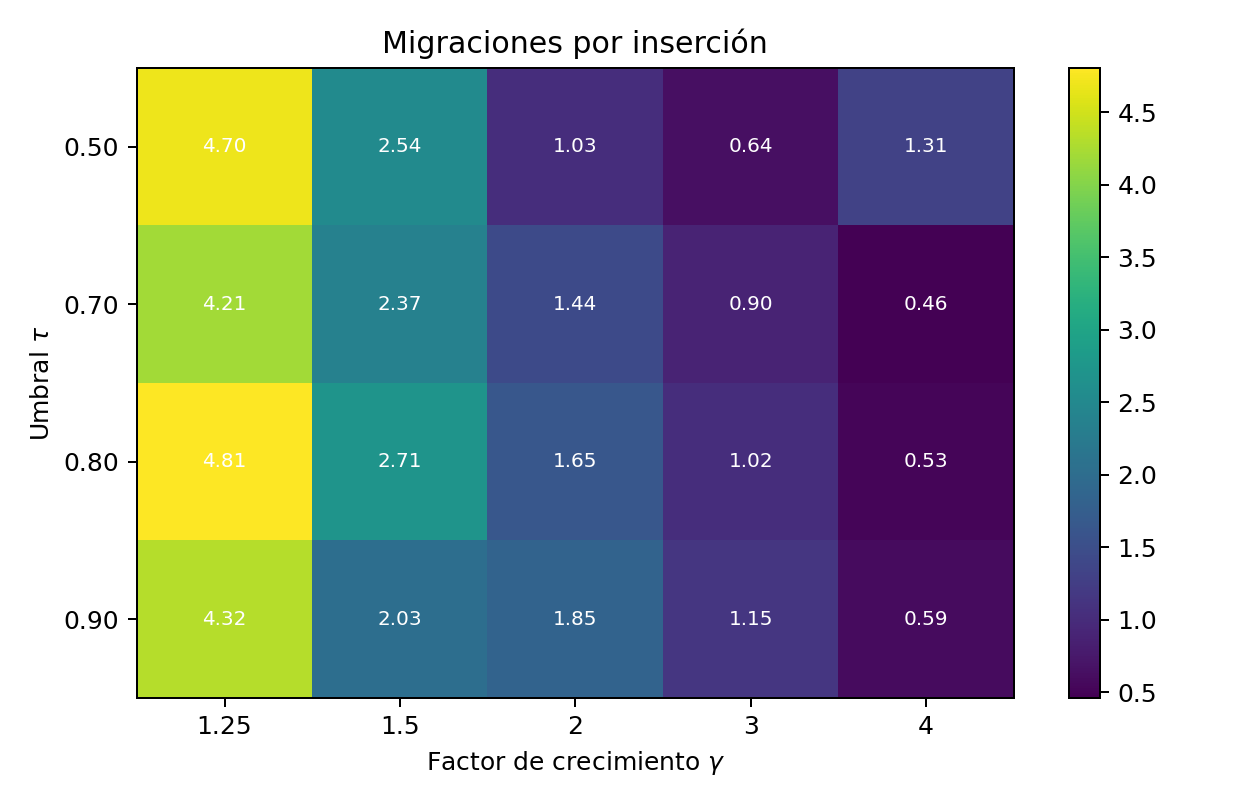
\includegraphics[width=.78\linewidth]{figuras/final/01_heatmap_migrations.png}
\caption{Migraciones por inserción para $N=100000$. Cada celda resume 30
semillas; el descenso general de izquierda a derecha respalda el efecto
amortizado esperado al aumentar $\gamma$.}
\label{fig:migraciones}
\end{figure}

El mapa también muestra por qué la predicción debe interpretarse de
manera agregada. La secuencia de capacidades es discreta y se redondea a
primos; además, el experimento se detiene exactamente en $N=100000$. Por
eso aparecen excepciones locales como $\tau=0.50$, donde $\gamma=4$
registra 1.31 migraciones por inserción frente a 0.64 con $\gamma=3$: el
último salto grande puede quedar cerca del final de la corrida y pesar
más en ese promedio particular. No obstante, la correlación de rangos
entre $\gamma$ y las migraciones agregadas es $-1.000$, y el número medio
de resizes desciende de 40.2 a 7.2 entre los extremos de $\gamma$. El
tiempo por operación acompaña esta tendencia: baja de 66080.8 a 27944.1
ns, aunque se considera una métrica secundaria porque incluye la
instrumentación de cada inserción.

La Figura~\ref{fig:pareto} completa la demostración al representar en una
misma vista las tres consecuencias de la política de crecimiento. El eje
horizontal mide migraciones por inserción, el vertical mide bytes
estructurales por elemento y el color codifica pares que colisionan por
clave. Por tanto, los tratamientos deseables se desplazarían hacia la
esquina inferior izquierda y, al mismo tiempo, tendrían colores asociados
con pocas colisiones. La nube no contiene un punto que reúna las tres
condiciones, lo que respalda la afirmación de H1 de que existe una
frontera de compromiso, no un ganador universal.

\begin{figure}[H]
\centering
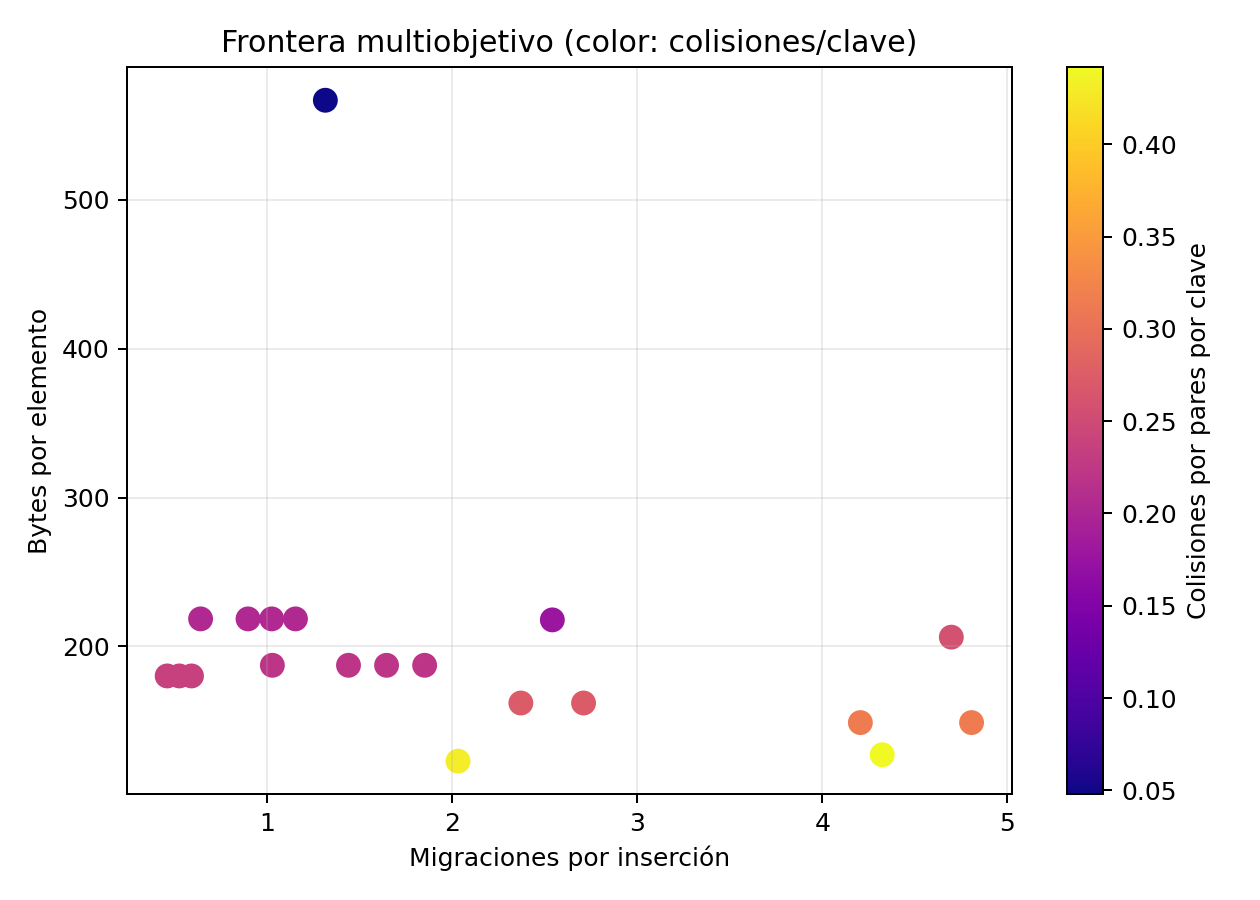
\includegraphics[width=.78\linewidth]{figuras/final/07_pareto.png}
\caption{Compromiso para $N=100000$: migraciones en el eje horizontal,
memoria en el vertical y colisiones por clave en el color. Ningún
tratamiento minimiza simultáneamente las tres métricas.}
\label{fig:pareto}
\end{figure}

Los extremos de la nube permiten cuantificar el intercambio. La menor
tasa de migración corresponde a $(\gamma,\tau)=(4,0.70)$, con 0.460
migraciones por inserción, 180.12 bytes por elemento y 0.236 pares por
clave. El menor uso de memoria aparece en $(1.5,0.90)$, con 122.86 bytes,
pero aumenta a 2.031 migraciones y 0.431 pares por clave. Finalmente,
$(4,0.50)$ logra la menor tasa de colisiones, 0.048, a costa de 566.99
bytes por elemento, el punto alto y aislado del gráfico. Estos casos
muestran que optimizar reconstrucciones, memoria o colisiones conduce a
elecciones diferentes.

El color también ayuda a interpretar el papel de $\tau$. Agregando sobre
$\gamma$, los pares por clave aumentan de 0.182 con $\tau=0.50$ a 0.307
con $\tau=0.90$; la correlación de rangos entre umbral y colisiones es
0.949. Esto respalda la segunda parte de H1: esperar más antes de crecer
tiende a mantener una tabla más cargada y eleva las colisiones. Sin
embargo, $\tau$ es un disparador y no determina por sí solo la carga
final. Dos políticas pueden alcanzar la misma capacidad prima y producir
resultados iguales, de modo que no se exige monotonía estricta en cada
tratamiento. Por la misma razón, estos resultados no permiten rechazar
H0 como afirmación causal una vez controlada exactamente la carga final.

Las 30 repeticiones por celda permiten atribuir estos patrones a la
política y no a una única función hash favorable. Como comprobación
adicional, para $N=100000$ el cociente medio entre pares observados y la
esperanza universal fue 0.964. El valor cercano a uno es coherente con el
modelo probabilístico, pero no se interpreta como una cota que deba
cumplirse en cada semilla.

El contraste de sondeo lineal contiene 540 corridas. Para $N=10000$, promediando factores de crecimiento y 30 semillas, los probes por inserción fueron 1.75, 3.46 y 8.26 para $\tau=0.50$, 0.75 y 0.90. Se informa como resultado separado porque su noción de colisión difiere de $C_{\mathrm{pares}}$.

\section{Discusión}
La caída de migraciones con $\gamma$ respalda la predicción amortizada $1/(\gamma-1)$. A la vez, el crecimiento de bytes por elemento muestra el precio espacial anticipado por $\gamma/\tau$. El mejor tratamiento depende, por tanto, de si se prioriza memoria, reconstrucciones o colisiones. La Figura~\ref{fig:pareto} hace visible esta ausencia de dominación total.

La correlación positiva entre $\tau$ y pares concuerda con la mayor carga. Sin embargo, $\tau$ es un disparador, no la carga final: el redondeo a primos y la trayectoria pueden hacer que dos políticas terminen con igual capacidad o presenten inversiones en un $N$ concreto. El cociente 0.964 frente a la cota universal es coherente en promedio, pero no prueba que cada ejecución deba quedar debajo de ella.

En sondeo lineal, el aumento de probes a alta carga concuerda cualitativamente con el análisis clásico \cite{FlajoletPobleteViola1998}. La diferencia de magnitud respecto del encadenamiento no indica por sí sola superioridad: las métricas, la representación de memoria y el mecanismo de resolución son distintos.

El tiempo por operación sigue en términos generales el volumen de migraciones, aunque incluye el costo de cronometrar cada inserción y mantener \texttt{tracemalloc}. Por eso las comparaciones bloqueadas dentro de este entorno son más defendibles que extrapolar nanosegundos absolutos a otra máquina.

\section{Limitaciones y amenazas a la validez}
La validez de constructo depende de no confundir eventos, pares, comparaciones y probes. La validez interna puede afectarse por GC, calentamiento y procesos del sistema; el bloqueo, la aleatorización y los contadores independientes del hardware reducen, pero no eliminan, esas amenazas. La medición con \texttt{sys.getsizeof} representa objetos de Python y no una tabla compacta en C.

La validez externa se limita a claves enteras únicas, ejecución monohilo, una familia modular y las distribuciones implementadas. Treinta semillas describen variabilidad, pero no convierten una muestra en demostración. Tampoco se evaluaron borrados, contracción ni adversarios adaptativos. Las referencias identificadas con asistencia de IA deben considerarse verificadas sólo cuando los integrantes hayan consultado sus fuentes originales y puedan defenderlas.

\section{Conclusiones y trabajo futuro}
La respuesta a la pregunta de investigación es que $\gamma$ y $\tau$ controlan un compromiso medible. En la implementación estudiada, crecer más redujo resizes y migraciones, pero aumentó la reserva de memoria; elevar el umbral aumentó la carga y, agregadamente, los pares que colisionan. H1 queda respaldada para las configuraciones y semillas ensayadas. H0 no puede rechazarse como afirmación causal después de controlar exactamente la carga, porque el factorial intervino políticas completas y no fijó $\alpha$ final de manera independiente.

No puede concluirse que $(\gamma,\tau)$ tenga un óptimo universal ni que los tiempos absolutos se trasladen a otras arquitecturas. Como trabajo futuro se proponen borrados con histéresis, contracción, claves adversas, otras familias hash y una implementación compacta que mida RSS y caché de hardware.

\section{Contribuciones y trazabilidad individual}
\begin{table}[H]
\centering\small
\caption{Responsabilidades y evidencia disponible al cierre documental.}
\begin{tabularx}{\linewidth}{p{3cm}p{3.5cm}X}
\toprule Integrante & Responsabilidad primaria & Evidencias principales \\
\midrule
José Cisternas & Integración, metodología y reproducibilidad & Commit \texttt{2efaf13}; \texttt{README.md}; protocolo y validación.\\
Gabriel Olarte & Contraste de sondeo lineal & Commit \texttt{69b5543}; adaptación en \path{src/linear_probing_hash_table.py}.\\
Bernardo del Aguila & Arquitectura modular y pruebas & Commit \texttt{524beb3}; \texttt{src/}, \texttt{tests/} y resultados preliminares.\\
Wara Murillo & Verificación bibliográfica y cobertura & Revisión asignada de anexos y papers núcleo; confirmación individual pendiente.\\
\bottomrule
\end{tabularx}
\end{table}

El equipo coordinó el trabajo mediante ramas y artefactos reproducibles. La tabla no sustituye las bitácoras separadas: cada integrante debe confirmar únicamente las tareas que realizó, corregir cualquier discrepancia y estar preparado para explicar la pregunta, algoritmos, metodología, resultados, matriz y conclusiones.

\section{Declaración de uso de IA}
\begin{table}[H]
\centering\footnotesize
\begin{tabularx}{\linewidth}{p{2.25cm}p{2.65cm}p{3.75cm}X}
\toprule Herramienta & Propósito & Prompt representativo & Verificación/modificación \\
\midrule
ChatGPT/Codex & Auditar ramas, apoyar código, análisis y LaTeX & ``Revisar \texttt{main} y \texttt{gabo}, integrar lo útil y crear entregables conforme a instrucciones e investigación.'' & Pruebas automatizadas, validación de CSV, compilación y revisión visual; el equipo debe revisar conceptos y atribuciones.\\
ChatGPT/Codex & Ajustar a las plantillas oficiales & ``Adaptar los entregables a las plantillas PDF oficiales de artículo y bitácora.'' & Se reprodujo orden, campos, tablas, apéndices y diagramación; se recompilaron cinco PDF.\\
\bottomrule
\end{tabularx}
\end{table}

La IA no se utilizó como fuente científica. Las referencias sugeridas se contrastaron con metadatos editoriales; la lectura profunda y la responsabilidad final corresponden a los estudiantes. Cada integrante debe comprender lo entregado y poder defender todas las filas de la Matriz Maestra.

\clearpage
\bibliographystyle{plain}
\bibliography{referencias}

\clearpage
\appendix
\section{Matriz Maestra de Cobertura Temática}
\small
\begin{longtable}{p{2.7cm}p{3.4cm}c p{6.2cm}}
\toprule
Unidad & Subtema & Estado & Justificación técnica y evidencia \\
\midrule\endfirsthead
\toprule Unidad & Subtema & Estado & Justificación técnica y evidencia \\\midrule\endhead
Análisis amortizado & Secuencias de operaciones & A & El costo se evalúa sobre secuencias completas de inserciones; Sec. 2.2 y CSV.\\
& Método agregado & A & Se suman migraciones de todos los resizes y se normalizan por $N$; Sec. 2.2.\\
& Método contable & P & Los créditos por inserción ofrecen una interpretación de cómo financiar migraciones; no es la prueba principal.\\
& Método potencial & P & Se discute como alternativa; ocupación sola no captura redondeo primo e interacción $(\gamma,\tau)$.\\
& Arreglos dinámicos & A & La reserva geométrica y frontera tiempo--espacio fundamentan el redimensionamiento; Sec. 2.3.\\
& Contadores y operaciones & A & Resizes ocasionales, elementos movidos y costo por operación están instrumentados en \texttt{src/}.\\
\midrule
Probabilidad y esperanza & Probabilidad básica & A & La elección de $(a,b)$ define el espacio aleatorio y los eventos de colisión.\\
& Esperanza matemática & A & Se contrasta $\mathbb{E}[C_{pares}]\le n(n-1)/(2m)$; Sec. 2.1 y Fig. 5.\\
& Variables indicadoras & A & Cada par aporta una indicadora; su suma produce $C_{pares}$ y permite linealidad de esperanza.\\
& Amortizado vs. esperado & A & Se distinguen explícitamente garantía de secuencia, esperanza sobre $h$ y media empírica.\\
\midrule
Algoritmos aleatorizados & Las Vegas & P & La tabla siempre conserva corrección; la función aleatoria afecta costo, no respuesta.\\
& Monte Carlo & N & No se acepta probabilidad de respuesta incorrecta: todas las inserciones se verifican.\\
& Probabilidad de error & N & No existe salida aproximada o errónea que deba amplificarse mediante repetición.\\
& Garantías de ejecución & P & Se comparan corrección determinista, costo amortizado y colisiones esperadas.\\
& Selección aleatoria & P & Se eligen aleatoriamente $(a,b)$ y el orden de tratamientos, no pivotes algorítmicos.\\
& Hashing universal & A & Es el mecanismo aleatorizado central; \texttt{src/universal\_hash.py}.\\
\midrule
P, NP y verificadores & Problemas de decisión & N & La pregunta estima rendimiento multiobjetivo, no decide un lenguaje sí/no.\\
& Certificados & N & Las observaciones no requieren testigo para una instancia ``sí''.\\
& Verificadores & N & No se formula certificado; la corrección se comprueba mediante invariantes polinomiales.\\
& Clase P & P & Inserción y validaciones tienen algoritmos polinomiales; no se estudia completitud.\\
& Clase NP & P & Se explica que pertenencia exige problema de decisión y verificador; esa forma no es central aquí.\\
& Decisión vs. optimización & P & Elegir una política Pareto es optimización multiobjetivo, distinta de una decisión formal.\\
\midrule
Reducciones y NP-completitud & Reducciones polinomiales & N & No se compara dificultad de lenguajes mediante transformaciones de instancias.\\
& Dirección de una reducción & N & No se afirma dureza; invertir una reducción no demostraría la implicación buscada.\\
& Prueba de NP-completitud & N & Faltan deliberadamente lenguaje, pertenencia a NP y reducción desde un problema base.\\
& SAT / 3-SAT & N & No modela la selección de parámetros ni la operación de la tabla.\\
& Clique & N & Las colisiones forman grupos por bucket, pero no equivalen a clique de una instancia arbitraria.\\
& Conjunto independiente & N & Evitar colisiones no se formula como selección de vértices sin adyacencias.\\
& Cobertura de vértices & N & No existe grafo de entrada ni objetivo de cubrir aristas.\\
& Ciclo hamiltoniano & N & La secuencia de buckets no exige visitar vértices una vez.\\
& Errores frecuentes & P & Se reconoce que una analogía estructural no constituye reducción ni equivalencia.\\
& Consecuencias prácticas & P & NP-completitud no implica que problemas polinomiales como esta simulación sean intratables.\\
\midrule
Aproximación & Algoritmos de aproximación & N & El factorial mide políticas; no aproxima una solución óptima NP-difícil.\\
& Razón de aproximación & N & La frontera de Pareto no ofrece razón demostrable respecto de un óptimo único.\\
& Análisis de garantías & P & Se analizan cotas amortizadas/esperadas, que no deben confundirse con garantía de aproximación.\\
\bottomrule
\end{longtable}
\normalsize


\clearpage
\section{Matriz bibliográfica}
\small
\begin{longtable}{p{2.5cm}p{3cm}p{3cm}p{3.4cm}p{2.8cm}}
\toprule
Fuente & Problema/objetivo & Método & Resultado relevante & Uso y limitación \\
\midrule\endfirsthead
\toprule Fuente & Problema & Método & Resultado & Uso/limitación \\\midrule\endhead
Carter--Wegman (1979) & Evitar supuestos benignos sobre claves & Familias universales y análisis probabilístico & Control de colisiones por pares & Fundamenta $C_{pares}$; no garantiza probes de sondeo lineal.\\
Tarjan (1985) & Costear secuencias con eventos caros & Análisis amortizado & Costo medio acotado sobre secuencias & Marco para migraciones; no prescribe $(\gamma,\tau)$.\\
Larson (1988) & Hashing dinámico en memoria & Diseño, análisis y experimentación & La expansión controla carga y reorganización & Paper núcleo más cercano; plataforma antigua.\\
Dietzfelbinger et al. (1994) & Hashing perfecto dinámico & Estructura aleatorizada multinivel & Consultas de peor caso y actualización esperada & Contraste teórico; estructura distinta.\\
Flajolet et al. (1998) & Costo del sondeo lineal & Combinatoria analítica & La carga cambia el régimen de probes & Respalda experimento secundario; no encadenamiento.\\
Brodnik et al. (1999) & Arreglos redimensionables eficientes & Diseño y análisis tiempo--espacio & Bajo espacio extra con acceso eficiente & Contexto de reserva; no tabla hash.\\
Pagh--Rodler (2004) & Búsqueda constante con dos posiciones & Cuckoo hashing & Rehash aleatorio ante ciclos & Relaciona aleatoriedad y reconstrucción; otro esquema.\\
Pătraşcu--Thorup (2012) & Independencia práctica del hash & Análisis de tabulación simple & Garantías dependen de la aplicación & Evita generalizar universalidad a todo probing.\\
Richter et al. (2015) & Comparar hashing multidimensionalmente & Benchmark experimental & No hay ganador universal & Motiva factorial y múltiples métricas.\\
Li et al. (2021) & Hash dinámico en GPU & Diseño concurrente y evaluación & Crecimiento depende de arquitectura & Fuente reciente; no extrapolable a Python.\\
Bender et al. (2022) & Sondeo lineal a alta carga & Análisis con tombstones & Reconstrucción y borrado cambian clustering & Contexto para probing; workload diferente.\\
Bender et al. (2023) & Optimizar varios criterios & Diseño y análisis de Iceberg hashing & Trade-offs simultáneos & Motiva Pareto; estructura más compleja.\\
Böther et al. (2023) & Hash vectorizado entre CPU & Benchmark multi-arquitectura & Hardware altera rankings & Amenaza externa; no prueba nuestra política.\\
Tarjan--Zwick (2024) & Arreglos redimensionables óptimos & Cotas y construcción & Frontera tiempo--espacio refinada & Paper núcleo reciente; no define política hash.\\
\bottomrule
\end{longtable}
\normalsize


\clearpage
\section{Registro de búsqueda bibliográfica}
\small
\begin{longtable}{p{2.3cm}p{1.7cm}p{4.2cm}p{3cm}p{3.45cm}}
\toprule Portal & Fecha & Consulta & Filtros & Resultado/estado \\
\midrule\endfirsthead
ACM DL & 08-09-2026 & ``universal classes hash functions'', ``dynamic hash tables'' & Fuente primaria, venue revisado & Carter--Wegman y Larson identificados; cada integrante debe confirmar lectura.\\
SIAM & 08-09-2026 & ``amortized computational complexity'', ``optimal resizable arrays'' & DOI/editor & Tarjan 1985 y Tarjan--Zwick 2024 identificados.\\
IEEE Xplore & 08-09-2026 & ``dynamic hash tables GPU'', ``linear probing tombstones'' & 2021--2026 & Li et al. y Bender et al. seleccionados como contexto reciente.\\
PVLDB & 08-09-2026 & ``analysis hashing methods'', ``vectorized hash tables CPU'' & Papers experimentales & Richter et al. y Böther et al. para metodología y amenazas.\\
SpringerLink & 08-09-2026 & ``linear probing analysis'', ``resizable arrays time space'' & DOI estable & Flajolet et al. y Brodnik et al. incorporados.\\
\bottomrule
\end{longtable}
\normalsize

\textbf{Nota de integridad.} Este registro fue estructurado con asistencia de IA a partir de la investigación suministrada. Antes de la entrega, los estudiantes deben abrir los DOI, consultar los trabajos y registrar en sus bitácoras qué secciones verificaron. Una referencia sugerida por IA no cuenta por sí sola como fuente consultada.


\section{Tres papers núcleo}
\begin{enumerate}[leftmargin=1.5em]
\item \textbf{Carter y Wegman (1979).} Problema: evitar supuestos sobre la distribución de claves. Método: familias universales y análisis probabilístico. Resultado: control esperado de colisiones por pares. Limitación: no implica cotas deterministas ni fórmulas de probing. Relación: fundamenta la variable $C_{\mathrm{pares}}$.
\item \textbf{Larson (1988).} Problema: expansión de tablas hash dinámicas. Método: diseño y evaluación de reorganización. Resultado: la política de crecimiento y la carga condicionan costo y espacio. Limitación: plataforma y estructuras diferentes. Relación: antecedente directo del factorial $(\gamma,\tau)$.
\item \textbf{Tarjan y Zwick (2024).} Problema: arreglos redimensionables con buen compromiso tiempo--espacio. Método: análisis y construcción algorítmica. Resultado: cotas refinadas para reserva dinámica. Limitación: no modela colisiones hash. Relación: contextualiza el costo espacial del crecimiento.
\end{enumerate}

\section{Control de bitácoras individuales}
\begin{table}[H]
\centering\small
\begin{tabularx}{\linewidth}{p{3.7cm}c X}
\toprule Integrante & Entregada & Archivo \\
\midrule
José Cisternas & Sí & \texttt{Jose\_Cisternas\_bitacora.pdf/.tex}\\
Gabriel Olarte & Sí & \texttt{Gabriel\_Olarte\_bitacora.pdf/.tex}\\
Bernardo del Aguila & Sí & \texttt{Bernardo\_del\_Aguila\_bitacora.pdf/.tex}\\
Wara Murillo & Sí & \texttt{Wara\_Murillo\_bitacora.pdf/.tex}\\
\bottomrule
\end{tabularx}
\end{table}
\end{document}
